\subsubsection{Functional Requirements}
\begin{itemize}
  \item The system must store all the account information.
  \item The user must be able to modify the password.
  \item The system must update any changed information.
  \item he system shall check that all the informations are valid.
\end{itemize}

\subsubsection{Scenario 1}
After five months that Susan is using PowerEnJoyshe she has decided that is better to change her \gls{pwd}. So she open her manage profile page and change it. Then she save the changes and the system upload Susan's information. Then for the future acesses Susan will use her new \gls{pwd}.

\subsubsection{Scenario 2}
Mark is a typical PowerEnJoy user. Unfortunatly his credic card is expired and so he has to change it. He was using that credit card also for pay his PowerEnJoy's charges. So as soon as he has his new credit card he decides to upload his payment information on PowerEnJoy. He accesses his manage profile page and changed the payment information. Since that moment PowerEnJoy is going to charge Mark on his new credit card.



\subsubsection{Mockups}
\begin{figure}[!ht]
  \centering
  \vspace{0.2cm}
  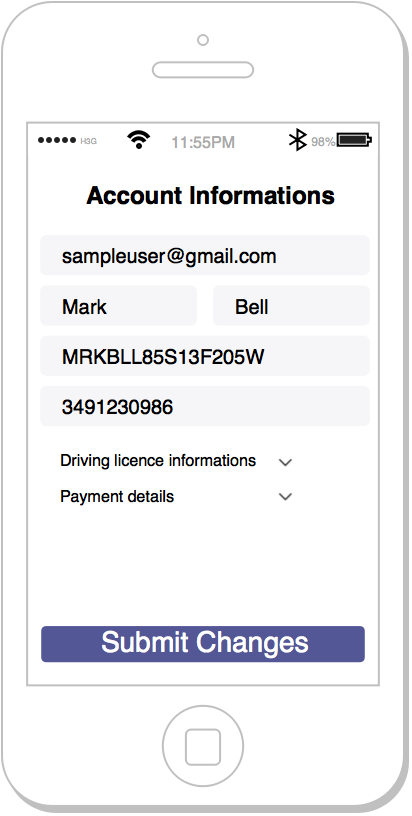
\includegraphics[width=0.25\textwidth]{/RASD/System_Functions/manage_account_mockup}\\
  \vspace{0.4cm}
  %\caption{Mockup for the account management mobile page} 
  \label{fig:manage_account_mockup} 
\end{figure}


\subsubsection{Use-case table}
\begin{center}
  \begin{tabular}{ l | p{10cm} }
    \hline
    Actors & User\\ \hline
    Goal & G\ref{itm:goal-account}\\ \hline
    Entry conditions & The User is logged into the system and she is viewing her profile page.   
    \\ \hline
    Flow of events &
      \begin{itemize}
        \item The User select the "Modify profile" option.
        \item The User modifies one or more information.
        \item The User submit the modifications.
        \item The system checks the modifications and upload them.
      \end{itemize} 
      \\ \hline
    Exit conditions & The User's profile is modified. \\ \hline
  Exceptions & 
\begin{itemize}
\item The User provides empty or invalid values as modifications (the system signals an error).
\item The User doesn't submit the modifications (the system aborts the request).
\item The system is not able to complete the operation due to some internal issues or connection broken (the system signals a ConnectionFailure).
\end{itemize} \\ \hline
  \end{tabular}
\end{center}


\subsubsection{Sequence diagram}
\begin{figure}[!ht]
  \centering
  \vspace{0.1cm}
  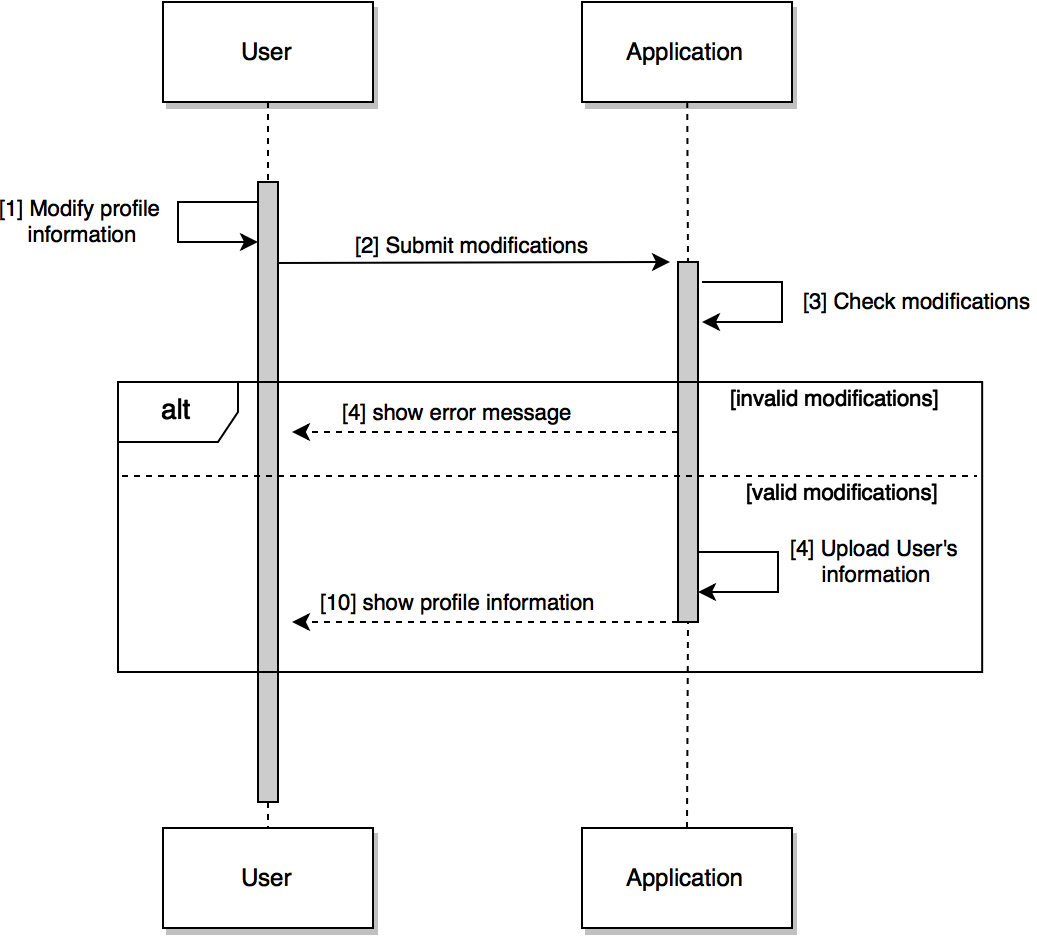
\includegraphics[width=0.55\textwidth]{/RASD/System_Functions/manage_account_sequence}\\
  \vspace{0.1cm}
  %\caption{Sequence diagram for the account management procedure} 
  \label{fig:manage_account_sequence} 
\end{figure}

